\section{Results}
\label{sec:formatting}

To interpret the performance of \(f_{\circ}\), we report the IoU metrics in table \ref{iou_results} that were computed by running \(f_{\circ}\) and \(f_c\) on \(\mathcal{X}_M\) and \(\mathcal{X}_{p}\). For each density, we calculate the IoU using the total set of pixels that \(f_{\circ}\) predicts as that density of smoke and the entire set of pixels labeled by the analyst as a particular smoke density over all imagery contained in the testing dataset. Additionally, we compute the overall IoU for all densities by first computing the number of pixels that intersect their corresponding density and divide that by the total number of pixels that make up the union of model predicted and analyst labeled smoke in the testing dataset.

\begin{table} 
    \caption{IoU results per density of smoke and over all densities using \(f_{\circ}\) and \(f_c\) with \(\mathcal{X}_M\) and \(\mathcal{X}_p\).}\label{iou_results}
    \centering
    \begin{tabular}{lcc|cc}
        \toprule
        \multicolumn{1}{c}{} & \multicolumn{2}{c}{\(f_{\circ}\)} & \multicolumn{2}{c}{\(f_c\)}\\
        \midrule
        \multicolumn{1}{c}{} & \(\mathcal{X}_M\) & \(\mathcal{X}_{p}\) & \(\mathcal{X}_M\) & \(\mathcal{X}_{p}\) \\
        \midrule
        Heavy   & 0.278 & 0.368 & 0.218 &  0.411 \\
        Medium  & 0.310 & 0.417 & 0.319 &  0.484 \\
        Light   & 0.480 & 0.585 & 0.491 &  0.660 \\
        Overall & 0.430 & 0.533 & 0.438 &  0.607 \\
        \bottomrule
    \end{tabular}
\end{table}

\begin{figure*}
    \centering
    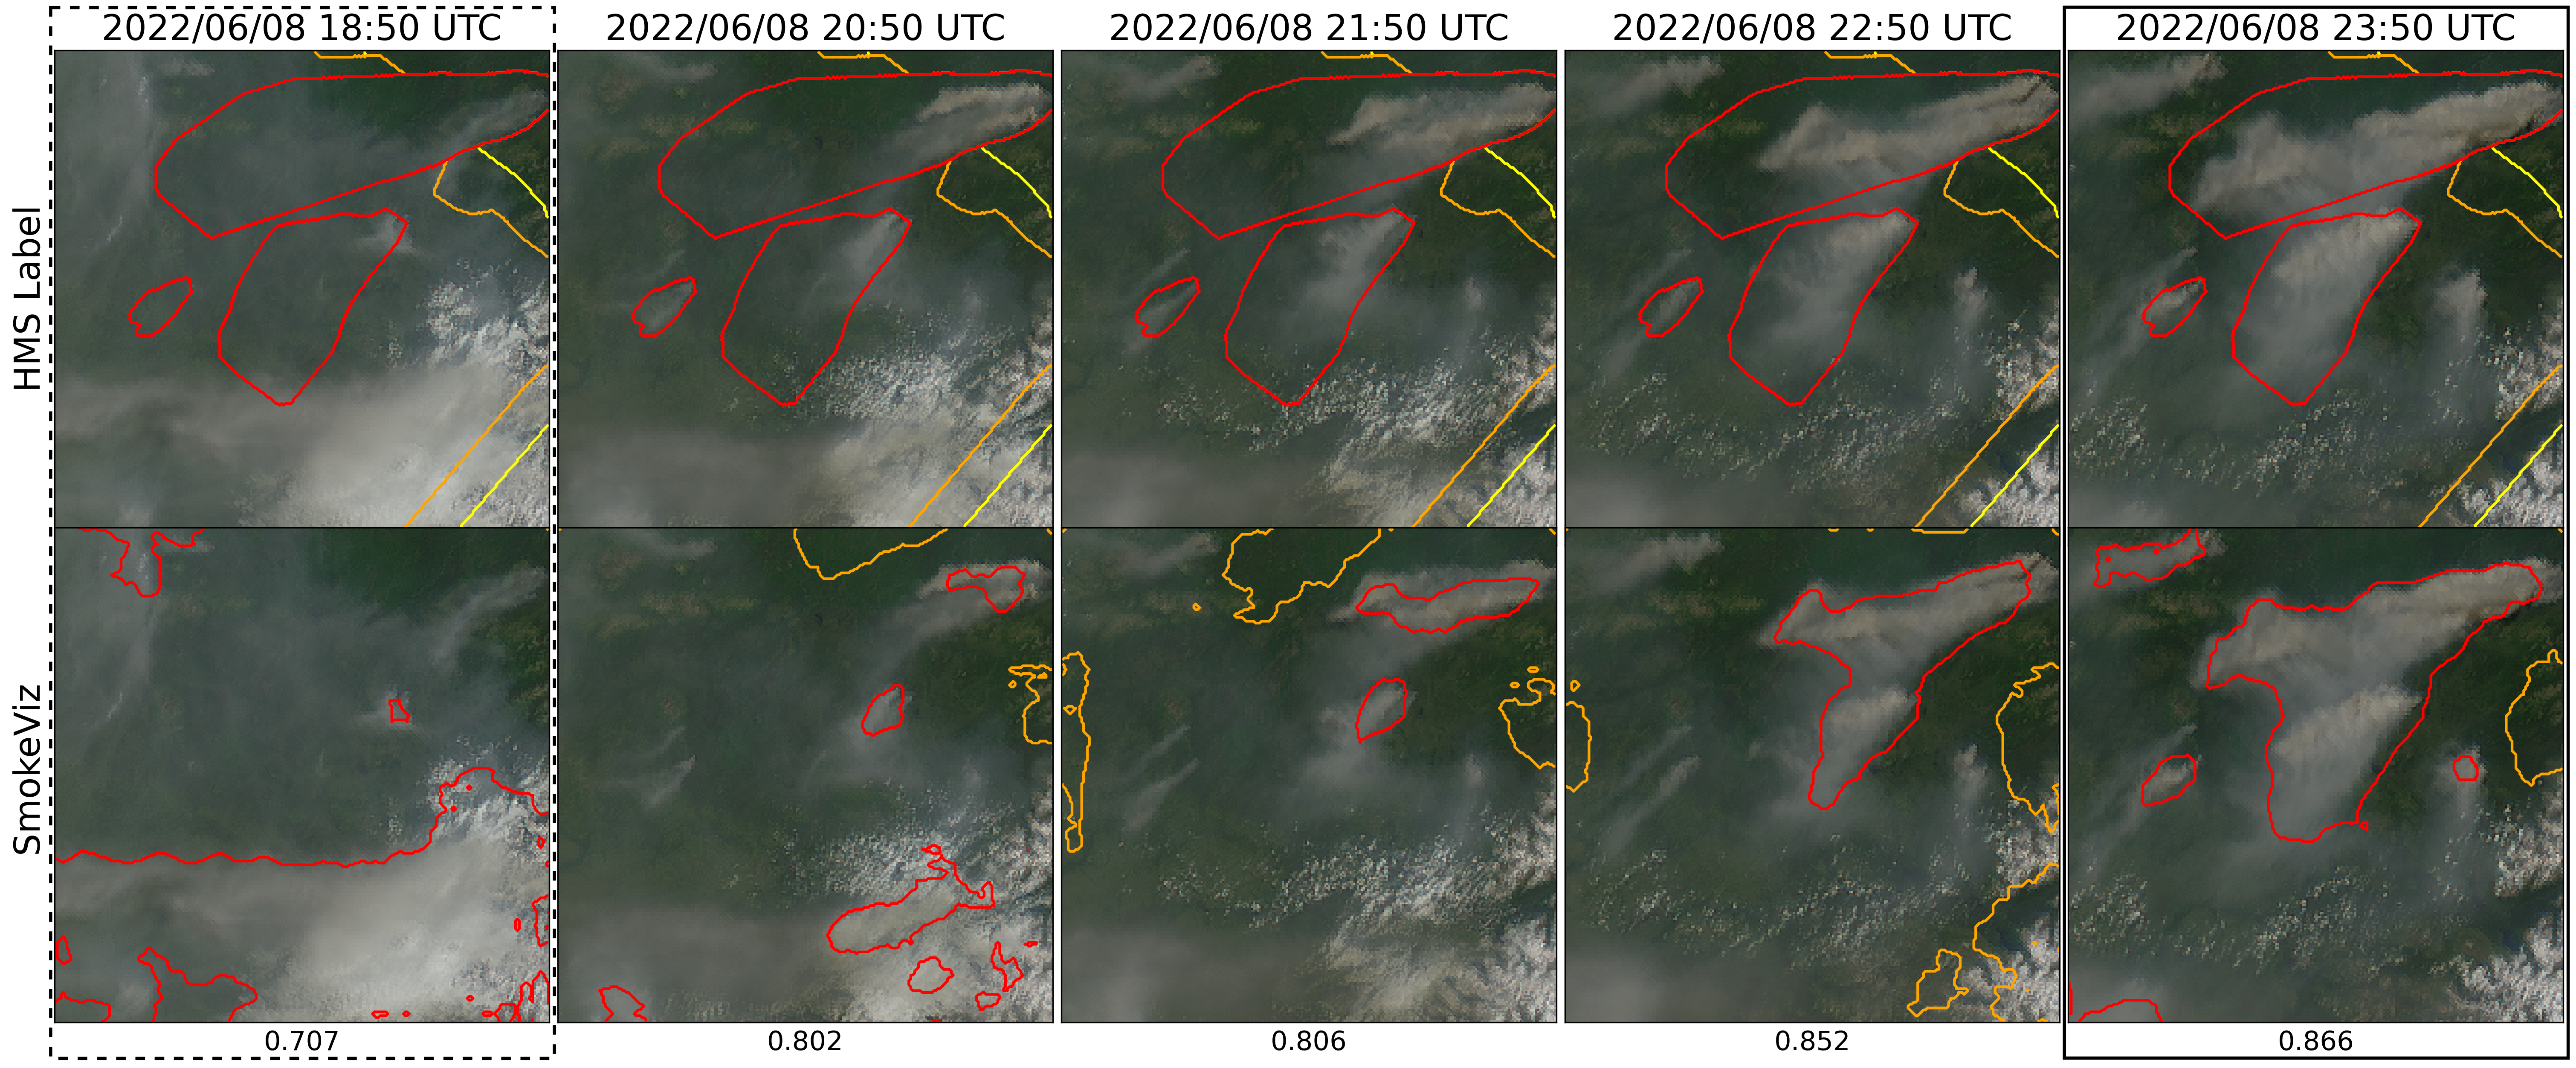
\includegraphics[width=17cm]{figures/final_results.png}
    \caption{GOES-West imagery showing smoke on June 8th, 2022 in Alaska where, at this geolocation (\(61.06^{\circ}\)N, \(156.12^{\circ}\)W), daylight was between 12:43-7:53 UTC. The HMS smoke annotations (top row) span from 18:50 to 23:50 UTC and are compared to the \(f_{\circ}\) generated pseudo-labels (bottom row). The first column (dotted outline) would be the GOES imagery selected for \(\mathcal{X}_{M}\) since it is closest to sunrise. The last column (solid outline) was selected for \(\mathcal{X}_{p}\) since it had the highest IoU value between the pseudo-label and analyst annotation. The IoU score over all densities is reported at the bottom of each column.}
    \label{ml_vs_mei}
\end{figure*}

An illustration of a pseudo-label picked image better representing the analyst annotation when compared to the Mie-derived image selection is evident in Figure \ref{ml_vs_mei}, where the heavy density smoke IoU increases from 0.01 to 0.59. The analyst annotation for these densities cover 5 hours of imagery, the Mie-derived selection optimizes for the image closest to sunrise while the pseudo-label image selection chooses the image with the highest overlap between the pseudo-label and the analyst annotation. The figure also illustrates how using a deep learning model can provide higher time resolution and give a dynamic representation of smoke over time.

To get an idea on how \(f_{c}\) compares to the HMS analyst annotations we show a series of samples from \(\mathcal{X}_{p}\) in figure \ref{bench}. The examples give a qualitative representation of how the predictions from \(f_c\) can provide more detailed boundaries of smoke densities than the HMS annotations do.

\begin{table}[h]
    \caption{Comparison of semantic segmentation model IoU performance on \(\mathcal{X}_{p}\).}\label{bench}
    \centering
    \begin{tabular}{cccrrcrc}
        \toprule
           & DLV3+ & MANet & PSPNet & Linknet \\
        \midrule
        Heavy   & 0.411 & 0.336  & 0.355 & 0.324 \\
        Medium  & 0.484 & 0.487  & 0.502 & 0.456 \\
        Light   & 0.662 & 0.675  & 0.690 & 0.662 \\
        Overall & 0.607 & 0.615  & 0.626 & 0.601 \\
        \bottomrule
    \end{tabular}
\end{table}

The results for the benchmarking models (table \ref{bench}) show similar performance across the models. DeepLabV3+ (\(f_c\)) gives the highest heavy density smoke IoU value, while PSPNet gives the highest overall IoU score.

\begin{figure*}
    \centering
    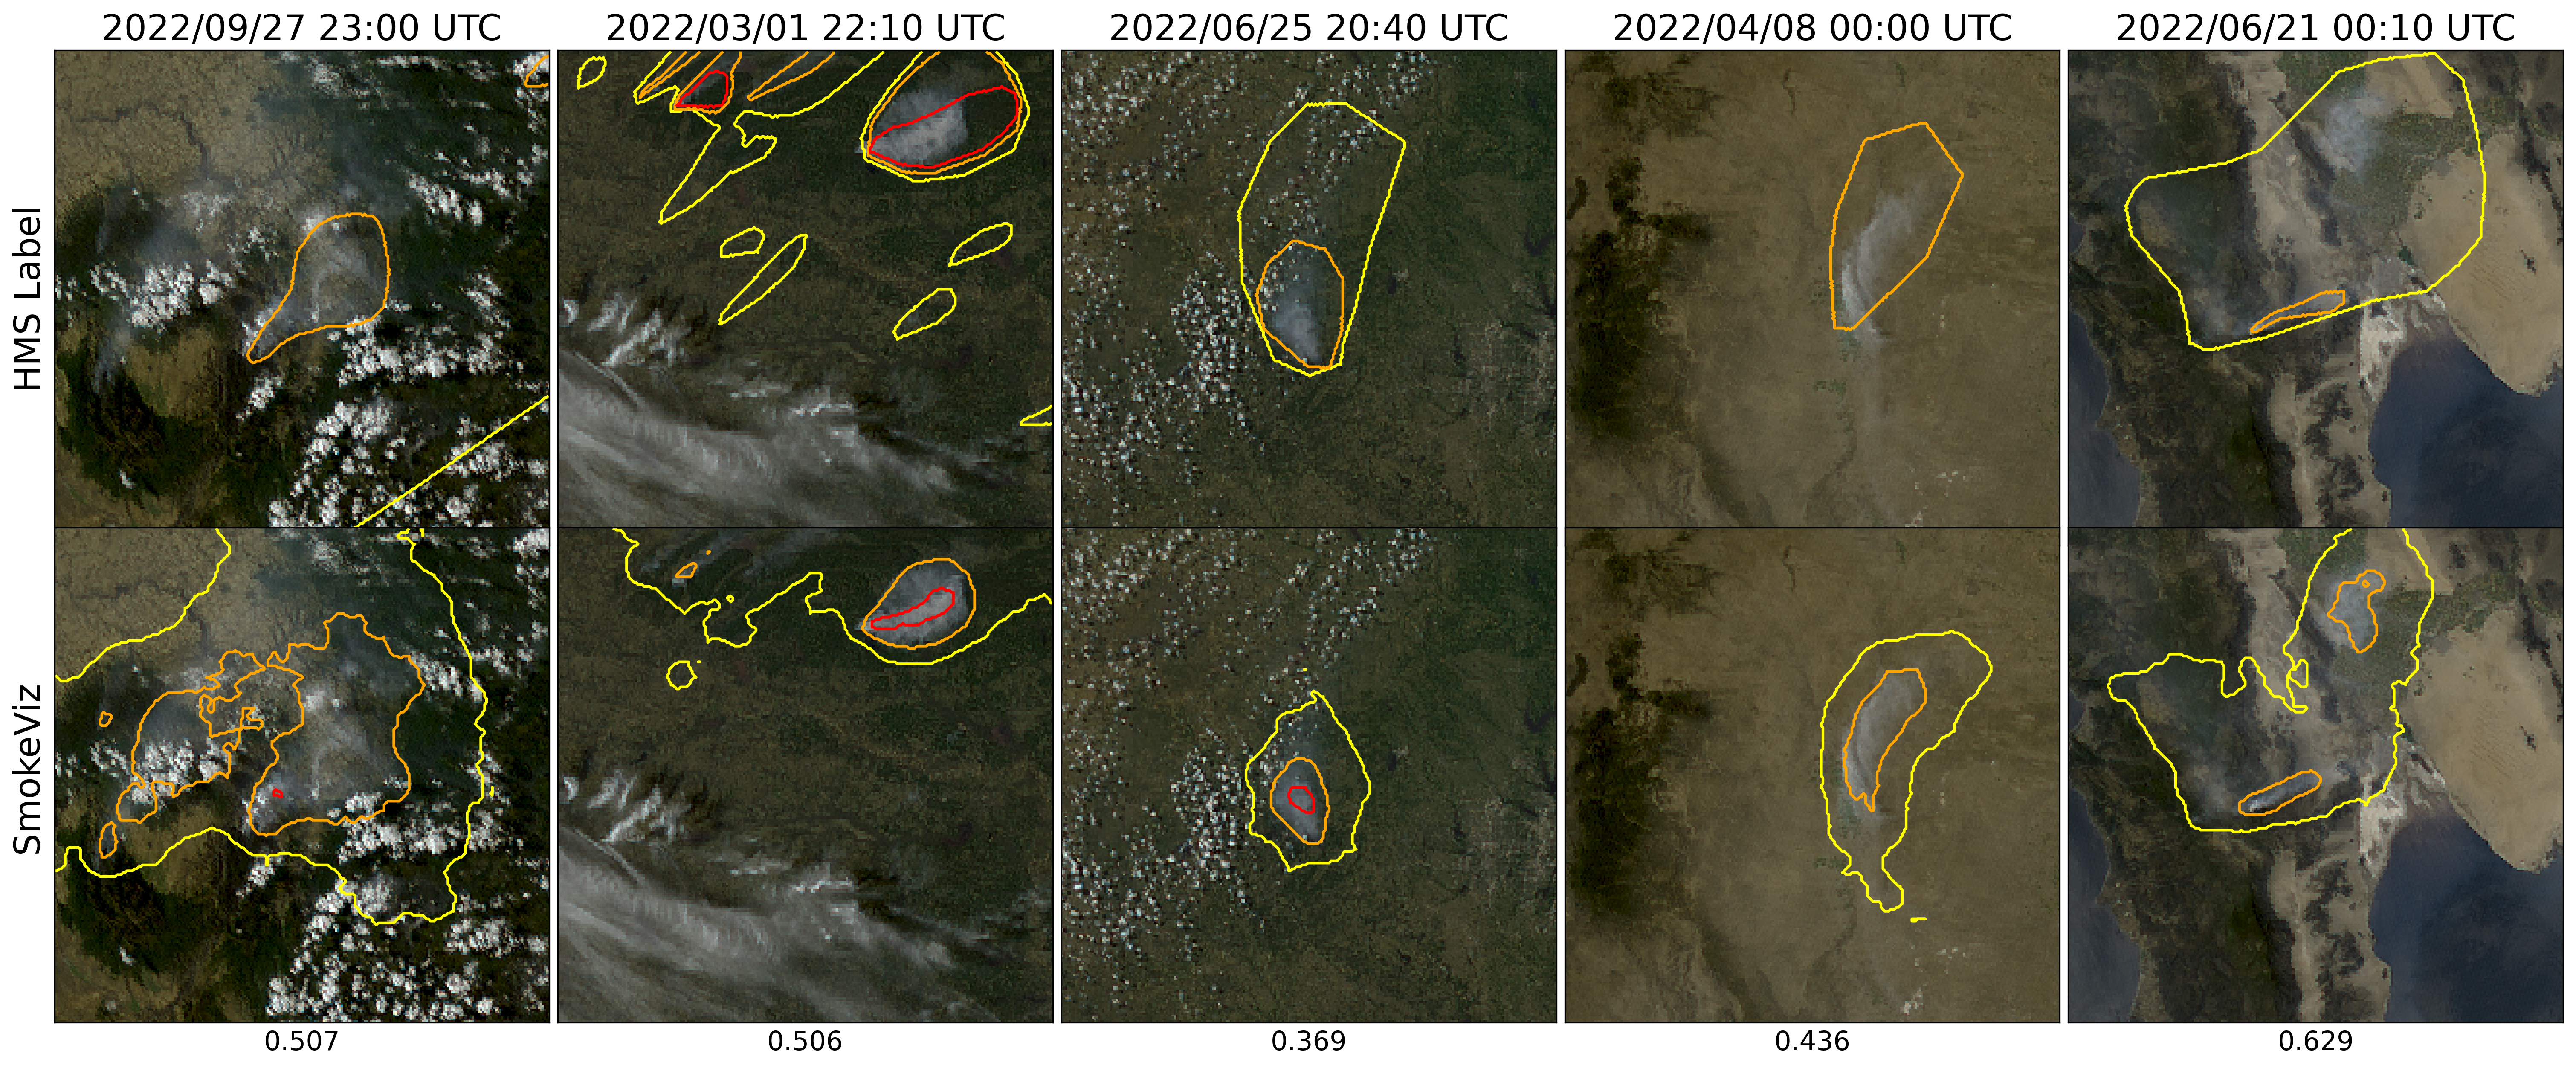
\includegraphics[width=17cm]{figures/examples.png}
    \caption{Examples of HMS annotations (top row) vs \(f_{c}\) output (bottom row) on \(\mathcal{X}_{p}\) samples. The overall IoU score is reported at the bottom of each column.}\label{examples}
\end{figure*}

\section{Limitations}

One of the concerns that comes with using pseudo-labeling methods is that you can perpetuate biases from the parent model into subsequent child models. Due to the increase in detectable forward scattered light off smoke particular matter, we expect the model to have a bias towards producing a higher success rate for smoke detection at larger solar zenith angles. The original HMS annotations do not distinguish by type of fire and include a large representation of controlled agricultural burns. This can be a limitation to consider if the dataset is being trained to target detection of large wildfires. All these limitations are discussed and analyzed further in the Appendix. Additional work should be done to analyze the performance of SmokeViz derived models on dust vs smoke.

\section{Conclusion}

In this study, we have refined an existing dataset originally curated by NOAA's HMS team, transforming it from a many-to-one imagery-to-annotation format to a more succinct, one-to-one satellite image-to-annotation dataset. The initial HMS dataset provided a general approximation of where smoke had been present for a given time window, though it did not guarantee the actual existence of smoke in the labeled pixels during the given times. Our goal was to create a dataset that could be used, along with additional applications, to train a model to detect wildfire smoke in real-time on an image-by-image level. The Mie-derived dataset selection process determined that if smoke was present, what timestamp within the analyst time window would the give the highest smoke signal-to-noise ratio. While optimizing for being able to detect smoke, if it is present, the Mie-dataset selection had no metric to determine if the smoke was effectually present in the selected image. Since many of the images within the HMS time-window either contained no smoke at all or the smoke was not contained within the geospatial bounds of the annotations, the Mie-derived dataset contained a large number of mislabeled samples. Discrepancies between data and labels can be detrimental towards the model's capacity to improve on feature representations in the target domain. During model training, the penalization of accurate predictions can inadvertently introduce biases towards misclassifying noise as meaningful signal. 

To improve the dataset's capacity to accurately represent wildfire smoke plumes, we train a parent machine learning model, \(f_{\circ}\), using the Mie-derived dataset, \(\mathcal{X}_M\), and run it on the relevant satellite images within the time-frame. The image with the maximum IoU score between the model's smoke predictions, or pseudo-label, and the analyst smoke annotations are used to create the pseudo-label generated dataset, \(\mathcal{X}_{p}\). We then train a child model, \(f_c\), using \(\mathcal{X}_{p}\) and test \(f_{\circ}\) and \(f_c\) on both the 2022 testing sets from \(\mathcal{X}_{M}\) and \(\mathcal{X}_{p}\). The results reported in table \ref{iou_results} suggest that \(\mathcal{X}_{p}\) was able to train a better performing model, \(f_c\), that gave higher IoU metrics on both dataset's testing sets in comparison to the original parent model, \(f_{\circ}\).

The result of this study is a representative dataset, SmokeViz, that can be used to train machine learning models for various wildfire smoke applications. A future goal is to produce a robust and reliable machine learning based approach for detecting wildfires using satellite imagery. That information can be used for wildfire detection and monitoring in along with a highly needed smoke product for data assimilation into smoke dispersion models. Additionally, this dataset can be used as a benchmark for how well remote sensing segmentation models can perform on dispersed edges such as smoke. On a broader scale, we show how pseudo-labeling can be used to optimize a dataset when the resolution for the data and corresponding labels do not match. This could be useful in similar applications involving time-series/video data with a singular label where the data can be compressed while still remaining representative of the label. All data is made publically available at [aws download link] and all code can be found at \url{https://github.com/anonymous-smokeviz/SmokeViz}.

